\chapter{Design}
This chapter summarizes the overall design of our approach to generating textual medical reports for X-ray images. The problem consists of multiple independent parts we need to deal with. For each of them, we we will present the fundamentals of our solution, along with description of related problematics and decisions made.

\section{Our approach}
As we already mentioned in the Chapter \ref{sec:RelatedWork}, the overall solution for the final medical report generation model is based on the \citet{alfarghaly2021automated}. We have chosen this approach for multiple reasons. The main reasons to use this work as the backbone for our thesis are following:
\begin{enumerate}
	\item In the work the state-of-the-art GPT-2 model is utilized as the language model. This gave us a great opportunity as there was none Czech GPT-2 model available at time this thesis began.
	\item The encoder is already fine-tuned to extract visual features for specific dataset.
	\item All solution source code is freely accessible on the github\footnote[1]{\url{https://github.com/omar-mohamed/GPT2-Chest-X-Ray-Report-Generation}}.
\end{enumerate}

As in most works for image captioning, the architecture is encoder-decoder based with an attention mechanism. The high-level solution architecture is depicted in Figure \hyperref[fig01:OmarArchitecutre]{2.1}.

\begin{figure}[h]\centering
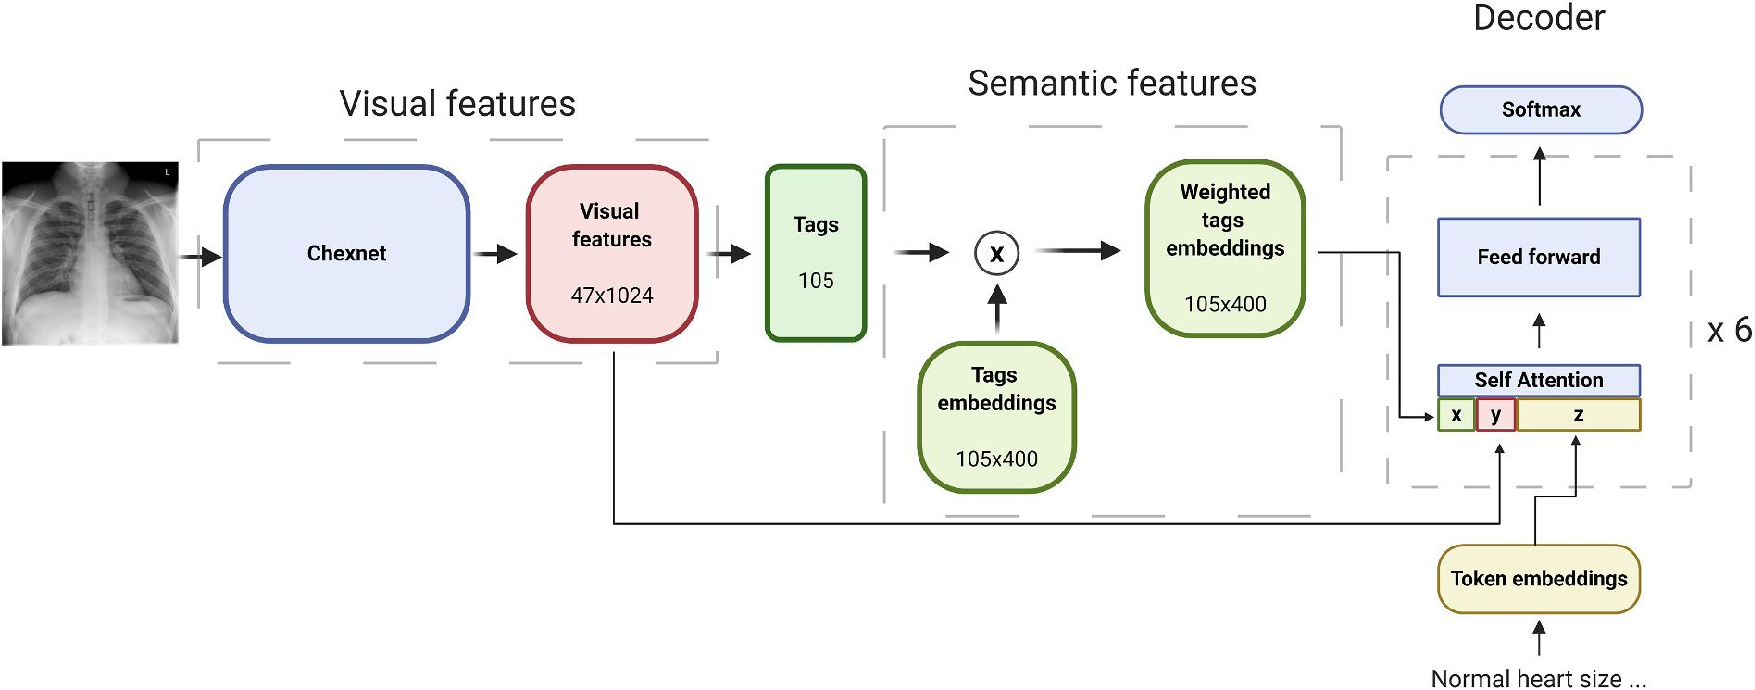
\includegraphics[width=145mm, height=57mm]{../img/OmarArchitecture}
\caption{Overall architecture used in our solution proposed in \citet{alfarghaly2021automated}.}
\label{fig01:OmarArchitecutre}
\end{figure}

\section{Czech GPT-2}
The aim of this work is to generate medical reports in the Czech language. In the previous parts, we decided to use the GPT-2 as the language model. However at the time of the beginning of this work, no Czech GPT-2 model was freely available and thus it was essentially necessary to create one. This section describes all the steps needed for fine-tuning the small English GPT-2 to the Czech language. Respectively, we train two versions of the Czech GPT-2 model. One trained on the general Czech textual data and one specialized specifically on Czech medical texts.

\subsection{Data}
In this section we will describe the possible data applicable for training of both the general and medical Czech GPT-2 model together with the decision made about the final data selection and data cleaning.

\subsubsection{General}
For the training of general Czech GPT-2 we have a plenty of data options we can choose from. However, there are important properties of the data we need to sastisfy. As we are transfer learning from English to Czech language we need to have sufficiently large data, so we ensure the GPT-2 will learn properly syntactical and semantical information. Moreover, the data have to be also heterogeneous enough, so the model can capture different types of information and not just for example newspaper articles from a specific area. In order to create a good enough general model we need to meet these criteria.\\

Several different dataset were investigated and tested for the training of the general Czech GPT-2 model.
\paragraph*{Czech Wikipedia} ~\\
\indent The first data we used for training the model is the Czech~Wikipedia~dump\footnote[2]{\url{https://dumps.wikimedia.org/cswiki/latest/cswiki-latest-pages-articles.xml.bz2}}. After extraction, the total size of the dataset is approximately 800 MB of raw text. The advantages of this dataset are its easy accessibility and fairly clean data quality. On the other hand, the data are very homogeneous despite the various topics. Each article is written in the general descriptive style. Moreover the data themself are not large enough, the trained model made many both syntactical and semantical mistakes during the text generation.

\paragraph*{Balanced Czech National Corpus} ~\\
\indent Another possibility was to use a balanced version of the Czech National Corpus\citep{11234/1-4635} as the original is composed mainly of journalistic articles. The balanced version tries to equalize the amount of data from each category. These categories include \textit{journalism}, \textit{poetry}, \textit{prose}, \textit{educational literature} etc. The major advantage of this dataset is its purity, the texts are syntacticaly correct without any undesirable non-Czech elements and written in the standard Czech language. The dataset does not have any significant downsides and the trained model understood Czech language without any significant ailments. In total, the dataset is comprised of 3,3 GB of raw text.

\paragraph*{OSCAR} ~\\
\indent OSCAR, from the \citet{ortiz-suarez-etal-2020-monolingual}, is a huge deduplicated multilingual corpus created from the Common~Crawl~corpus\footnote[3]{\url{https://commoncrawl.org/}} providing data for 166 different languages and available directly in the huggingface datasets library\footnote[4]{\url{https://huggingface.co/datasets/oscar}}. It consists of the text scraped from websites of very different kinds and thus the data are heteregeneous enough. Moreover, its huge size, as the czech part of the dataset occupies a total of 24 GB of raw text, is another major benefit. On the other hand, because the data are automatically scraped, they carry a noise in them. Besides that, not negligible part of the text are in the non-standard Czech language as the data come from diverse web sources such as forums etc. Nevertheless, the disadvantages are outweighed by the huge size of the corpus and together with following filtering of the text:
\begin{enumerate}
	\item We take only text that are at least 1200 characters longs as these texts tend to be longer articles written in the standard Czech language instead of advertisements, incomple texts etc.
	\item Any text containing control character are filtered out, because the text contains generally undesirable content.
\end{enumerate}

\paragraph*{Conclusion} ~\\
\indent We analyzed various datasets along with their overall properties. Furthermore, the advantages and disadvantages of each were discussed. As a result, we have chosen the \textbf{OSCAR} dataset due to its size and heterogeneity. The \textbf{Wikipedia} is too small and homogeneous. On the other hand the \textbf{Balanced Czech National Corpus} is heterogeneous enough, however it is an almost order of magnitude smaller than \textbf{OSCAR}.

\subsubsection{Medical}
Since we have a trained general Czech GPT-2 model from the previous section that already understands a Czech language, the final fine-tuning for medical environment does not require that much data. We need to specialize the model to understand the mecial environment inherently. For this purpose, we use a subset of the UFAL~Medical~Corpus~v. 1.0\footnote[5]{\url{https://ufal.mff.cuni.cz/ufal\_medical\_corpus}}. These data are further filtered to remove any inappropriate characters, lines and redundant structures. As a result, the data contain a total of 100 MB of raw medical texts. The texts comprise of general medical descriptions, articles and package leaflets for medicines.

\subsection{Training}
Popsat postup tréninku podle příspěvku + learning rate finder + diff lear. rates + ta trénovací křivka

\section{Medical dataset translation}
Alpha and omega of the final model
\subsection{Translator choice}
\subsection{Preprocessing}



